%%%%(c)
%%%%(c)  This file is a portion of the source for the textbook
%%%%(c)
%%%%(c)    Abstract Algebra: Theory and Applications
%%%%(c)    Copyright 1997 by Thomas W. Judson
%%%%(c)
%%%%(c)  See the file COPYING.txt for copying conditions
%%%%(c)
%%%%(c)


\chap{Symmetries of Plane Figures\quad
\sectionvideohref{8wveTstkSfU&index=18&list=PL2uooHqQ6T7PW5na4EX8rQX2WvBBdM8Qo}}{symmetries}

\begin{quote}
``In all the arts it is symmetry that gives pleasure, preserving unity, and making the whole beautiful.'' (Augustine, \emph{Of True Religion}, xxx.55 (Tr. J. H. S. Burleigh)
\end{quote}
\begin{quote}
``It is only slightly overstating the case to say that physics is the study of symmetry.'' (Philip W. Anderson, 1977 Nobel laureate in physics)
\end{quote}
\begin{quote}
``So our problem is to explain where symmetry comes from. Why is nature so nearly symmetrical? No one has any idea why.'' (Richard Feynman, 1965 Nobel laureate in physics)
\end{quote}

The above quotes give some flavor of the importance and the mystery of symmetry, in both art and science. In keeping with our practice throughout this book, we will introduce this general topic by means of a basic example, namely symmetries of plane figures. Many of the concepts that you will learn in this chapter are applicable to symmetries in general. In particular: wherever you find a symmetry, you will always find a \emph{group} lurking behind it (see Section~\ref{DefOfGroup} for the mathematical definition of a group).
\medskip

Thanks to Tom Judson for material used in this chapter.


\section{Definition and examples}

In plane geometry we talk about various shapes: triangles, rectangles, pentagons, and so on. Shapes are important because real objects have shapes (duh), and objects are important. What would life be without triangles?

Now suppose you and your friend cut an equilateral triangle out of a piece of plane white paper and put it on the table. Then you tell your friend to go out of the room. While she's gone, you take the triangle and move it, but in such a way that it looks exactly the same. You can do this by rotating the triangle, or flipping it over, or by some combination of these two actions. When your friend comes back into the room, although the triangle has been moved there's no way for her to tell. This type of motion is called a \emph{symmetry operation}. Clearly we may perform symmetry operations on other objects besides equilateral triangles, but only if the shape of the object has some kind of regularity. In the following discussion, we will explore the relationship between shapes and symmetry operations. 

We've given an intuitive picture of what symmetry means--now let's try to translate that into mathematics. We start with a definition:

\begin{defn} A \term{symmetry}\index{Symmetry!definition} of a geometrical figure is a rearrangement of the figure that (i) preserves distances and angles between points of the figure,
 and (ii) leaves the appearance and location of the figure unchanged.
\end{defn}

\begin{rem}
The meaning  of ``preserves distances'' can be expressed more precisely as follows. Take any two points $A$ and $B$ of the original figure. The figure is then rearranged so that $A$ and $B$ are sent to points $A'$ and $B'$ respectively. Then in order for the rearrangement to be  a symmetry, the distance between $A$ and $B$ must always be equal to the distance between $A'$ and $B'$.

Similarly, the meaning of  ``preserves angles'' can be expressed more precisely as follows. Take any three points $A, B, C$ of the original figure. The figure is then rearranged so that $A, B, C$ are sent to $A', B', C'$ respectively. In order for the rearrangement to be  a symmetry, $\angle ABC$ must always be equal to $\angle A'B'C'$ regardless of the choice of $A, B, C$.
\footnote{It can be shown mathematically that a rearrangement that preserves distances must necessarily preserve angles as well. So strictly speaking, the additional  angle preservation  requirement is not necessary.}
\end{rem}

A motion that preserves distances and angles between parts of a figure is also called a \term{rigid motion}\index{Rigid motion}. Intuitively, you may think of the figure as a rigid object, and the ``rearrangement'' is effected by moving the rigid object in some fashion.  For example, any \term{rotation}\index{Rotation! as rigid motion}  that does not change the shape of the object is a rigid motion.

\begin{figure}[ht]
\begin{center}
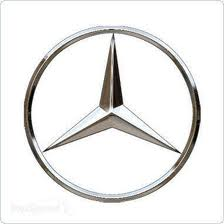
\includegraphics[scale=0.35]{images/mercedes.jpg}
\caption{Mercedes Logo}\label{mercedes}
\end{center}
\end{figure}

\begin{example}{mercedeslogo} Consider the Mercedes logo shown in Figure~\ref{mercedes}.
\begin{itemize}
\item
Imagine pinning the center of the logo to the page and spinning the logo $120^\circ$ counterclockwise about its center. The resulting image looks exactly like the original, because each of the three points on the circumference moves  to the location of the next point over. So a $120^\circ$ counterclockwise rotation is a symmetry of the logo. 
\item
If you rotate the image $180^\circ$ counterclockwise about the center, the resulting image is no longer identical to the original (try it!).  So a $180^\circ$ counterclockwise rotation is not a symmetry of the logo.  
\item
We could also ``flip over'' the logo (like flipping a pancake) in such a way that the left half moves to the right, and vice versa.  Then the vertical point stays in the same place while the left and right point exchange positions, leaving the appearance of the logo unchanged. The motion has the same effect as if the logo were \term{reflected} across the vertical axis.\index{Reflection (rigid motion)} After the motion, the logo looks the same. 
\item
Shifting  the original image (shifts are also called \term{translations}\index{Translation!as a rigid motion} in any direction is a rigid motion, and  the resulting image looks the same as the original, but the location is different.  Hence this shift is \emph{not} not a symmetry of the Mercedes logo.
\end{itemize}
\end{example}

\begin{exercise}{mercedes}
List six different symmetries of the Mercedes logo.
\hyperref[sec:symmetries:hints]{(*Hint*)}
\end{exercise}

This is not the first time we've played with symmetries of a figure.  At the end of Chapter 1, we saw that the complex sixth roots of unity determined a regular hexagon in the complex plane, and that complex multiplication and complex conjugation could be used to rotate or reflect the hexagon. 
Let us investigate the hexagon a bit further.

\begin{example}{hexagon}
Figure~\ref{hex60rot}  shows a $60^\circ$ counterclockwise rotation of a regular hexagon where the vertices of the hexagon are labeled $A,B,C,D,E,F$. (Notice how the letters run \emph{counterclockwise} around the hexagon. We will consistently follow this pattern. The reason is that in mathematical convention, a counterclockwise rotation is considered as \emph{positive}, while a clockwise rotation is considered as \emph{negatve}.)


\begin{figure}[ht]
\begin{center}
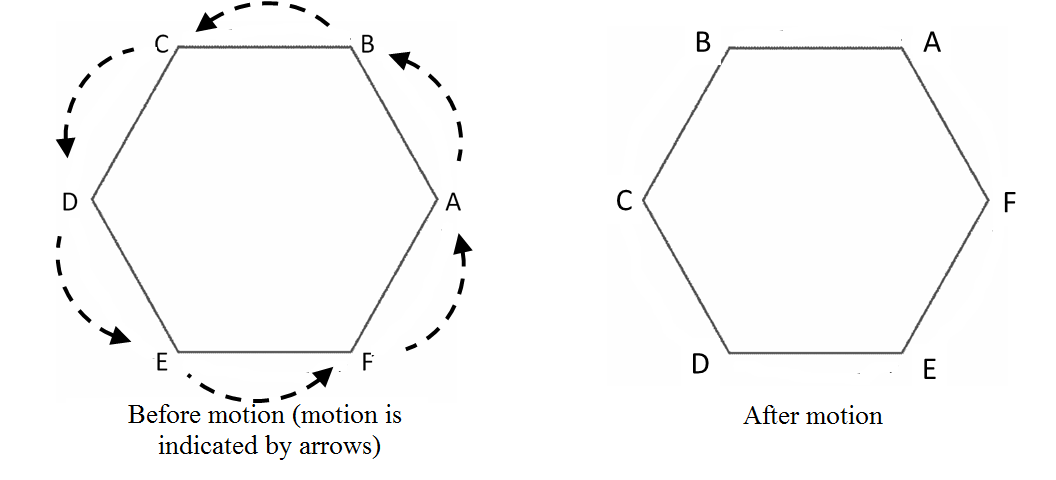
\includegraphics[width=5in]{images/hexABCDEF_1.png}
\caption{\label{hex60rot} Hexagon and  $60^\circ$ rotation}
\end{center}
\end{figure}



The rotation moves $A$ to $B$, $B$ to $C$, and so on.  Now of course there are other points on our figure, namely all the points on the line segments between the vertices.  But notice that if we account for where the vertices are moved to, then the movement of the line segments is automatically accounted for.  If we know where $A$ and $B$ are moved to, we know exactly where $\overline{AB}$ is.  Therefore, our $60$ degree rotation can be defined by the movement of the vertices  $\{A,B,C,D,E,F\}$.  

Now if we input a point from $\{A,B,C,D,E,F\}$, our rotation outputs a point from $\{A,B,C,D,E,F\}$.  We have used this ``input-output" language before, namely in the Functions chapter. 

In fact, we can think of the $60$ degree rotation as a function $r_{60}$ from $\{A,B,C,D,E,F\} \to \{A,B,C,D,E,F\}$, where (using ordered pair notation)
\[r_{60} = \{ (A,B), (B,C), (C,D), (D,E), (E,F), (F,A) \}.\]
Before leaving this example, we make note of a peculiarity that has tripped up many a student. If you compare the 'before' hexagon (shown at left in Figure~\ref{hex60rot}) with the `after' hexagon (shown at right), it appears that the original vertex $B$ has been relabeled as' $A$, $C$ has been relabeled as $B$, and so on.  However, according to our function we say that $A$ goes to $B$, not $B$ goes to $A$. This is because we're thinking of symmetry as a \emph{motion} rather than a relabeling. The fact that original vertex $B$ is relabeled as $A$ means that $A$ moved to $B$, and not vice versa. So you should take care in future examples--whenever you see a vertex $X$ being relabeled as $Y$ this means that $Y \rightarrow X$, and not vice versa.\footnote{Actually, we could have defined symmetries as relabelings rather than motions, and all of the conclusions of this chapter would still hold. We'd just have to rewrite all of our tableaus to reflect this different convention.}

 

\end{example}

\begin{exercise}{hexagon}
\begin{enumerate}[(a)]
\item
Is $r_{60}$ one-to-one?  Explain why or why not.
\item
Is $r_{60}$ onto?  Explain why or why not.
\item
Is $r_{60}$ a bijection?  Explain why or why not.

\end{enumerate}
\end{exercise}

Exercise~\ref{exercise:symmetries:hexagon} exemplifies a general property of symmetries:

\begin{prop}{SymmBijection}  
If $S$ is the set of points that represent a figure, all symmetries of the figure are bijections from $S \to S$.
\end{prop}

\begin{proof}
Since the result of any symmetry acting on $S$ must be all of $S$, then every point of $S$ must be in the range of $S$. Thus any symmetry is onto. Furthermore, the symmetry must map two different points to two different points, since the distance between points must be left unchanged by the symmetry. Hence any symmetry is one-to-one.  So since any symmetry is both onto and one-to-one, it follows that any symmetry is a bijection.
\end{proof}
\medskip

Proposition~\ref{proposition:symmetries:SymmBijection} says that all symmetries are bijections, but the \emph{converse} is not true: all bijections are not symmetries. 

\begin{exercise}{bijectnotsym}
 Create a bijection from $\{A,B,C,D,E,F\} \to \{A,B,C,D,E,F\}$ that does not correspond to a symmetry of the regular hexagon in  Figure~\ref{hex60rot}. \emph{Explain} why it is not a symmetry.
\end{exercise}

\begin{example}{rectsymmetries}
Figure~\ref{SymmOfRect} below shows all symmetries of a rectangle.

\begin{figure}[htb]   %Symmetries of a rectangle  Replaced diagram with a tikz figure - TWJ 5/4/2010
\begin{center}
\tikzpreface{groups_rectangle}
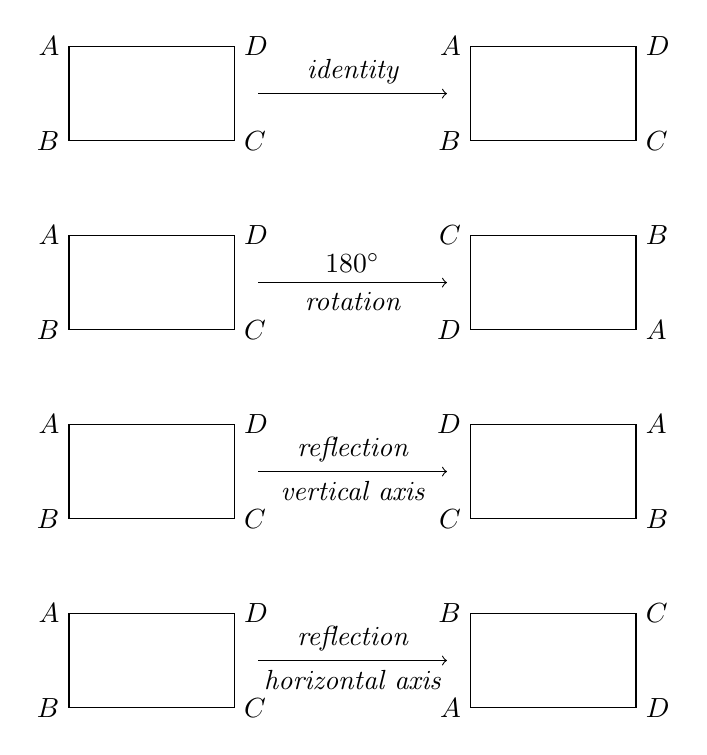
\begin{tikzpicture}[scale=1.2]\label{groups_figure_rectangle}
\draw (-3,0) -- (-1.25,0) -- (-1.25,1) -- (-3,1) -- cycle;
\draw (3,0) -- (1.25,0) -- (1.25,1) -- (3,1) -- cycle;
\draw [->] (-1,0.5) -- (1,0.5);
\node [above] at (0,0.5) {{\em reflection}};
\node [below] at (0,0.5) {{\em horizontal axis}};
\node [above,left] at (-3,1) {$A$};
\node [below,left] at (-3,0) {$B$};
\node [above,right] at (-1.25,1) {$D$};
\node [below,right] at (-1.25,0) {$C$};
\node [above,right] at (3,1) {$C$};
\node [below,right] at (3,0) {$D$};
\node [above,left] at (1.25,1) {$B$};
\node [below,left] at (1.25,0) {$A$};

\draw (-3,2) -- (-1.25,2) -- (-1.25,3) -- (-3,3) -- cycle;
\draw (3,2) -- (1.25,2) -- (1.25,3) -- (3,3) -- cycle;
\draw [->] (-1,2.5) -- (1,2.5);
\node [above] at (0,2.5) {{\em reflection}};
\node [below] at (0,2.5) {{\em vertical axis}};
\node [above,left] at (-3,3) {$A$};
\node [below,left] at (-3,2) {$B$};
\node [above,right] at (-1.25,3) {$D$};
\node [below,right] at (-1.25,2) {$C$};
\node [above,right] at (3,3) {$A$};
\node [below,right] at (3,2) {$B$};
\node [above,left] at (1.25,3) {$D$};
\node [below,left] at (1.25,2) {$C$};

\draw (-3,4) -- (-1.25,4) -- (-1.25,5) -- (-3,5) -- cycle;
\draw (3,4) -- (1.25,4) -- (1.25,5) -- (3,5) -- cycle;
\draw [->] (-1,4.5) -- (1,4.5);
\node [above] at (0,4.5) {$180^\circ$};
\node [below] at (0,4.5) {{\em rotation}};
\node [above,left] at (-3,5) {$A$};
\node [below,left] at (-3,4) {$B$};
\node [above,right] at (-1.25,5) {$D$};
\node [below,right] at (-1.25,4) {$C$};
\node [above,right] at (3,5) {$B$};
\node [below,right] at (3,4) {$A$};
\node [above,left] at (1.25,5) {$C$};
\node [below,left] at (1.25,4) {$D$};

\draw (-3,6) -- (-1.25,6) -- (-1.25,7) -- (-3,7) -- cycle;
\draw (3,6) -- (1.25,6) -- (1.25,7) -- (3,7) -- cycle;
\draw [->] (-1,6.5) -- (1,6.5);
\node [above] at (0,6.5) {{\em identity}};
\node [above,left] at (-3,7) {$A$};
\node [below,left] at (-3,6) {$B$};
\node [above,right] at (-1.25,7) {$D$};
\node [below,right] at (-1.25,6) {$C$};
\node [above,right] at (3,7) {$D$};
\node [below,right] at (3,6) {$C$};
\node [above,left] at (1.25,7) {$A$};
\node [below,left] at (1.25,6) {$B$};

\end{tikzpicture}
\caption{\label{SymmOfRect}Symmetries of a rectangle}
\end{center}
\end{figure}
\end{example}

\begin{exercise}{10}
\begin{enumerate}[(a)]
\item
Explain why a $90^\circ$ rotation, a $270^\circ$ rotation, or reflection across a diagonal are not symmetries  of the rectangle $ABCD$.
\item
What subcategory of rectangle would have a $90^\circ$ rotation, $270^\circ$ rotation, and a reflection across a diagonal as symmetries?
\item
What rotation angle does the identity symmetry correspond to? (Give the easiest answer.)
\item
Write each of the symmetries of a rectangle as a function (use either a table, ordered pairs, arrow diagram, etc.)
\end{enumerate}
\end{exercise}  


\section{Composition of symmetries}

Since the symmetries of a figure are functions, we can do anything with symmetries that we can do with functions--including composition.  That is,  we can perform two symmetries on a figure back-to-back, and since they are both functions, by definition of function composition the result is a function.  In fact, we saw in the Functions chapter that the composition of two bijections is a bijection.  So the composition (or net motion) resulting from two symmetries is a bijection.  But a bijection of a figure is not necessarily a symmetry. as we showed in Exercise~\ref{exercise:symmetries:bijectnotsym} above.  This raises the question:  is the composition of two symmetries a symmetry?  That is: if one symmetry is followed by another on a figure, is the net motion a symmetry?  You will investigate this question in the following exercise.

%A natural question to ask is what happens to a figure if one symmetry is followed by another?  Is the net motion a symmetry?  Or do we come up with some other motion of the figure that is not a symmetry?  Lets think about this question in terms of functions.  Since symmetries are functions, performing two symmetries back to back corresponds to composing two functions.  By definition, the composition of two functions is a function.  Further, from Exercise~\ref{functions:exercise:BijectionComposeExer} (a) in the Functions chapter, we know that the composition of two bijections is a bijection.  However, from Exercise~\ref{symmetries:exercise:bijectnotsym} above, we know all bijections aren't necessarily symmetries.  So the composition of two symmetries is a bijection, but the question remains:  is the composition of two symmetries a symmetry?

\begin{exercise}{SymmComposition}
With reference to the symmetries of a rectangle in Example~\ref{example:symmetries:rectsymmetries}, let  $r_{180}$ be the $180^\circ$ counterclockwise rotation and let $s_v$ be the reflection across the vertical axis.
(Note that reflection across the vertical axis is sometimes called ``horizontal reflection,'' since the figure ``flips'' from left to right. Admittedly this is confusing, but that's what people call it so what can you do?)
\begin{enumerate}[(a)]
\item
Write the function $r_{180}$ in ordered pair notation.
\item
Write the function $s_v$ in ordered pair notation.
\item
Write the function $r_{180} \compose s_v$ in ordered pair notation. Is it a symmetry of the rectangle? If so, then which one?
\item
Write the function $s_v \compose r_{180}$ in ordered pair notation. Is it a symmetry of the rectangle? If so, then which one?
\end{enumerate}
\end{exercise}
 
At this point let us introduce an alternative notation for symmetries that's easier to write.  This notation is called \term{tableau form}, and for $r_{180}$ it looks like the following:
\medskip

$r_{180} = \begin{pmatrix} A & B & C & D \\ C & D & A & B \end{pmatrix} $
\medskip

To form these, we simply put the inputs of our function on the top row and their corresponding outputs on the bottom row.  

\begin{example}{sym_tableau}
For example, since 

\[ s_v = \{(A, D), (B,C), (C, B), (D, A) \}, \]

\noindent
then the top row of the tableau for $s_v$ would read, ``$A  B  C  D$", and the bottom row of the tableau would read, ``$D  C  B  A$".  Hence  

\[ s_v = \begin{pmatrix} A & B & C & D \\ D & C & B & A \end{pmatrix}. \]
\end{example}

\begin{example}{sym_comp_tableau}
Suppose we wanted to find  $r_{180} \compose s_v$ using the tableau forms for $r_{180}$ and $s_v$ above.  That is

\[ r_{180} \compose s_v = \begin{pmatrix} A & B & C & D \\ C & D & A & B \end{pmatrix} \compose  \begin{pmatrix} A & B & C & D \\ D & C & B & A \end{pmatrix} = ? \]

\noindent
To see how this works, let's ``follow" each possible input ($A, B, C, D$) as we put it into the composition.   Remember that the composition of functions works right to left; we are first reflecting the rectangle and then rotating it.  So starting from the right, 
\begin{itemize}
\item
$ s_v$ takes $A \to D$, and $r_{180}$ takes $D \to B$.  Therefore $r_{180} \compose f_h$ takes $A \to B$; i.e. $(r_{180} \compose s_v)(A) = B$.
\item
$ s_v$ takes $B \to C$, and $r_{180}$ takes $C \to A$; therefore $r_{180} \compose s_v$ takes $B \to A$
\item
$ s_v$ takes $C \to B$, and $r_{180}$ takes $B \to D$; therefore $r_{180} \compose s_v$ takes $C \to D$
\item
$ s_v$ takes $D \to A$, and $r_{180}$ takes $A \to C$; therefore $r_{180} \compose s_v$ takes $D \to C$
\end{itemize}
\noindent
Figure~\ref{fig:ChangingRoom} shows this process using tableaus.  If you think about it, it's really just a variation on an arrow diagram.
\begin{figure}[ht]
\begin{center}
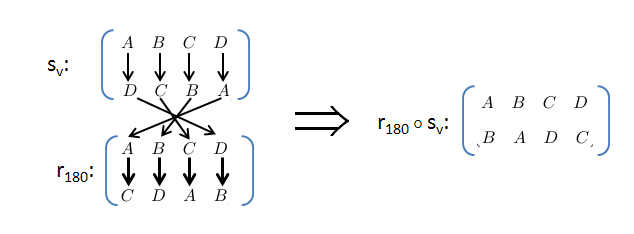
\includegraphics[scale=0.6]{images/ChangingRoom.png}
\caption{Composition of symmetries using tableaus.}\label{fig:ChangingRoom}
\end{center}
\end{figure}
\noindent

In summary we have

\[ r_{180} \compose s_v = \begin{pmatrix} A & B & C & D \\ C & D & A & B \end{pmatrix} \compose  \begin{pmatrix} A & B & C & D \\ D & C & B & A \end{pmatrix} = \begin{pmatrix} A & B & C & D \\ B & A & D & C \end{pmatrix} \]
 \end{example}

\begin{exercise}{CompSymm}
\begin{enumerate}[(a)]
\item
Write $s_h$ in tableau form, where $s_h$ is reflection across the horizontal axis. (Note $s_h$ is sometimes referred to  as ``vertical reflection,'', since the two reflected halves are stacked on top of each other.)
\item
Does $r_{180} \compose s_v = s_h$?
\item
Compute $s_h \compose  s_v$. Is this a symmetry? If so, which one?
\item
Compute $s_v \compose r_{180}$.  Is this a symmetry? If so, which one?
\end{enumerate}
\end{exercise}

\noindent
Exercises~\ref{exercise:symmetries:CompSymm} and~\ref{exercise:symmetries:SymmComposition} seem to indicate that the composition of two symmetries of a figure is a symmetry of the figure. We can actually prove that this is always true.

\begin{prop}{symcompclosed}
Suppose $f$ and $g$ are both symmetries of a figure.  Then $f \compose g$ is itself a symmetry of the same figure.
\end{prop}

\begin{proof}
Recall that composition works from right to left. Since $g$ is a symmetry, $g$ takes the points of the figure and rearranges them so that the angles and distances of points in the figure are preserved.  The symmetry$f$ then takes the points of this preserved figure and moves them in such a way that the angles, and distances of points in the figure are preserved.  Hence the net result of $f \compose g$ preserves angles and distances between points in the figure.  Therefore by definition, $f \compose g$ is a symmetry of the figure.
\end{proof}

\begin{exercise}{16}
With reference to the hexagon in Figure~\ref{hex60rot}, for the symmetries $f$ and $g$ in parts (a)-(d) below:
\begin{enumerate}[(i)]
\item
Write the symmetries $f$ and $g$ in tableau form.
\item
Compute $f \compose g$ and $g \compose f$, expressing your answers in tableau form.
\item 
Describe the symmetries that correspond to $f \compose g$ and $g \compose f$, respectively.
\end{enumerate}
\medskip

\noindent
Note ${\var id}$ denotes the identity symmetry, that is the symmetry that leaves all points unchanged.
\medskip

\begin{enumerate}[(a)]
\item
$f=$ rotation by $240^\circ, g=$ rotation by $120^\circ$
\item
$f={\var id}, g=$ rotation by $120^\circ$
\item
$f=$rotation by $ 240^\circ, g=$reflection across the line $BE$
\item 
$f=$rotation by $ 180^\circ, g=$reflection across the line $CF$
\end{enumerate}
\end{exercise}

\section{Do the symmetries of an object form a group?\quad
\sectionvideohref{EC5do5EUQ9c&index=19&list=PL2uooHqQ6T7PW5na4EX8rQX2WvBBdM8Qo?}}\label{SymmetryGroup}

With reference to the set of symmetries of a particular figure,  Proposition~\ref{proposition:symmetries:symcompclosed} tell us that this set is closed under the operation of composition. Given this fact, the next natural inquiry is to see if this set of symmetries forms a group under composition.  Let's look first at a particular example to see if it works.

\begin{example}{symmsofeqtri}
Figure~\ref{groups_s3_symmetry_fig} shows all the symmetries of an equilateral triangle:  ${\var id}$ is the identity  ; $\rho_1$ is the $120^\circ$ counterclockwise rotation; $\rho_2$ is the $240^\circ$ counterclockwise rotation; $\mu_1$ is the reflection across the median through $A$; $\mu_2$ is the reflection across the median through $B$; and $\mu_3$ is the reflection across the median through $C$. We remind the reader once again of the comment we made in Example~\ref{example:symmetries:hexagon}: for example, in the symmetry $\rho_1$ the triangle's vertices $A,B,C$ before the motion appear to be relabeled as $C,A,B$ respectively, which means that $C \rightarrow A$, $A \rightarrow B$, and $B \rightarrow C$ rather than vice-versa.

\begin{figure}[htp] %Replaced diagram with a tikz figure - TWJ 5/5/2010
\begin{center}
\tikzpreface{groups_s3_symmetry}
\begin{tikzpicture}[scale=0.7]
\draw (0,0) -- (0:2) -- (60:2) -- cycle;
\node [left] at (0,0) {$A$};
\node at (1,2.1) {$C$};
\node [right] at (0:2) {$B$};

\draw [->] (2,1) -- (4,1);
\node [above] at (3,1) {{\em reflection}};

\draw (4,0) -- (0:6) -- ++(120:2) -- cycle;
\node [left] at (4,0) {$B$};
\node [right] at (0:6) {$A$};
\node at (5,2.1) {$C$};

\node [right] at (7,1) {$ \mu_3 = \begin{pmatrix} A & B & C \\ B & A & C \end{pmatrix}$};

\draw (0,3) -- (2,3) -- ++(120:2) -- cycle;
\node [left] at (0,3) {$A$};
\node at (1,5.1) {$C$};
\node [right] at (2,3) {$B$};

\draw [->] (2,4) -- (4,4);
\node [above] at (3,4) {{\em reflection}};

\draw (4,3) -- (6,3) -- ++(120:2) -- cycle;
\node [left] at (4,3) {$C$};
\node [right] at (6,3) {$B$};
\node at (5,5.1) {$A$};
\node [right] at (7,4) {$ \mu_2 = \begin{pmatrix} A & B & C \\ C & B & A \end{pmatrix}$};

\draw (0,6) -- (2,6) -- ++(120:2) -- cycle;
\node [left] at (0,6) {$A$};
\node at (1,8.1) {$C$};
\node [right] at (2,6) {$B$};

\draw [->] (2,7) -- (4,7);
\node [above] at (3,7) {{\em reflection}};

\draw (4,6) -- (6,6) -- ++(120:2) -- cycle;
\node [left] at (4,6) {$A$};
\node [right] at (6,6) {$C$};
\node at (5,8.1) {$B$};
\node [right] at (7,7) {$ \mu_1 = \begin{pmatrix} A & B & C \\ A & C & B \end{pmatrix}$};

\draw (0,9) -- (2,9) -- ++(120:2) -- cycle;
\node [left] at (0,9) {$A$};
\node at (1,11.1) {$C$};
\node [right] at (2,9) {$B$};

\draw [->] (2,10) -- (4,10);
\node [above] at (3,10) {{\em rotation}};

\draw (4,9) -- (6,9) -- ++(120:2) -- cycle;
\node [left] at (4,9) {$B$};
\node [right] at (6,9) {$C$};
\node at (5,11.1) {$A$};
\node [right] at (7,10) {$ \rho_2 = \begin{pmatrix} A & B & C \\ C & A & B \end{pmatrix}$};

\draw (0,12) -- (2,12) -- ++(120:2) -- cycle;
\node [left] at (0,12) {$A$};
\node at (1,14.1) {$C$};
\node [right] at (2,12) {$B$};

\draw [->] (2,13) -- (4,13);
\node [above] at (3,13) {{\em rotation}};

\draw (4,12) -- (6,12) -- ++(120:2) -- cycle;
\node [left] at (4,12) {$C$};
\node [right] at (6,12) {$A$};
\node at (5,14.1) {$B$};
\node [right] at (7,13) {$ \rho_1 = \begin{pmatrix} A & B & C \\ B & C & A  \end{pmatrix}$};

\draw (0,15) -- (2,15) -- ++(120:2) -- cycle;
\node [left] at (0,15) {$A$};
\node at (1,17.1) {$C$};
\node [right] at (2,15) {$B$};

\draw [->] (2,16) -- (4,16);
\node [above] at (3,16) {{\em identity}};

\draw (4,15) -- (6,15) -- ++(120:2) -- cycle;
\node [left] at (4,15) {$A$};
\node [right] at (6,15) {$B$};
\node at (5,17.1) {$C$};
\node [right] at (7,16) {$ {\var id} = \begin{pmatrix} A & B & C \\ A & B & C  \end{pmatrix}$};

\end{tikzpicture}
\end{center}
\caption{Symmetries of an Equilateral Triangle}
\label{groups_s3_symmetry_fig}
\end{figure}
\end{example}

\noindent
Table~\ref{S3_table} displays  all possible compositions of the symmetries shown in Figure~\ref{groups_s3_symmetry_fig}. The table is arranged like a multiplication table: for example, the table entry in the row marked ``$\rho_1$'' and the 
column marked ``$\mu_1$'' corresponds to the composition $\rho_1 \compose \mu_1$.  From now on we will refer to all such tables as \term{Cayley tables}, regardless of the operation being represented (addition, multiplication, composition, \ldots)

\begin{table}
{\small
\begin{center}
\begin{tabular}{c|cccccc}
$\circ$  & ${\var id}$     & $\rho_1$ & $\rho_2$ & $\mu_1$ & $\mu_2$ & $\mu_3$ \\
\hline
${\var id}$     & ${\var id}$     & $\rho_1$ & $\rho_2$ & $\mu_1$ & $\mu_2$ & $\mu_3$ \\
$\rho_1$ & $\rho_1$ & $\rho_2$ & ${\var id}$     & $\mu_3$ & $\mu_1$ & $\mu_2$ \\
$\rho_2$ & $\rho_2$ & ${\var id}$     & $\rho_1$ & $\mu_2$ & $\mu_3$ & $\mu_1$ \\
$\mu_1$  & $\mu_1$  & $\mu_2$  & $\mu_3$  & ${\var id}$    & $\rho_1$& $\rho_2$\\
$\mu_2$  & $\mu_2$  & $\mu_3$  & $\mu_1$  & $\rho_2$& ${\var id}$    & $\rho_1$\\
$\mu_3$  & $\mu_3$  & $\mu_1$  & $\mu_2$  & $\rho_1$& $\rho_2$& ${\var id}$
\end{tabular}
\end{center}
}
\caption{Composition of the symmetries of an equilateral triangle}
\label{S3_table}
\end{table}

\begin{rem}
NOTE it is very easy to get mixed up with Cayley tables for the composition operation. When \emph{looking up} the value of $f \compose g$, you use the row headings for $f$ and the column headings for  $g$, but when \emph{computing} $f \compose g$, it is $g$ that is applied first and then $f$.
\end{rem}

\begin{exercise}{S3Table}
Verify the following entries in Table~\ref{S3_table} by (i) writing the symmetries in tableau form and (ii) computing the composition directly.
\begin{enumerate}[(a)]
\item
Row 2, column 4
\item
Row 4, column 2
\item
Row 3, column 6
\item
Row 6, column 3
\end{enumerate}
\end{exercise}

\begin{exercise}{20}
Use Table~\ref{S3_table} to answer the following questions. 
\begin{enumerate}[(a)]
\item
Explain why Table~\ref{S3_table} shows that ${\var id}$ satisfies the definition of an identity element.
\item
Does every element in $S$ have an inverse?  List the inverses for each symmetry that has an inverse.
\item
Explain why Table~\ref{S3_table} shows that composition is \emph{not} commutative.
\end{enumerate}
\end{exercise}

So far so good.  The composition operation on $S$ has closure, an identity, and inverses for each element.  There is one more group property left to check -- the associative property. It is difficult to check this property on the Cayley table of $S$; we would have to prove it for all 3-symmetry combinations in $S$, which would be a bit exhausting.\footnote{In mathematics, there is a type of proof called ``proof by exhaustion,'' but this is typically a last resort. One famous mathematician (George Polya) once said, "Mathematics is being lazy. Mathematics is letting the principles do the work for you so that you do not have to do the work for yourself."}  
However, luckily we can prove the symmetries of any figure are associative in general.

\begin{prop}{symcompassoc}
The set of symmetries $S$ of any figure under composition is associative.
\end{prop}

\begin{proof}
By definition, we know any symmetry of a figure is a function.  From the Functions chapter, we know that composition of functions is associative.  Therefore for any three symmetries $s_1, s_2, s_3 \in S$, by the associative property of functions, 
\[ \bigl( s_1 \compose s_2 \bigr) \compose s_3 = s_1 \compose \bigl( s_2 \compose s_3 \bigr). \]

\noindent
Therefore $S$ is associative under composition.
\end{proof}
\medskip

Tada!  The set of symmetries of an equilateral triangle are indeed a group under function composition.  
\medskip

We've managed to prove this for one example; what about for the set of symmetries of any figure?  Could we prove the set of symmetries of any figure are a group under composition?  We've already proved the closure and associative properties hold for any figure (Propositons~\ref{proposition:symmetries:symcompassoc} and ~\ref{proposition:symmetries:symcompclosed}).  Now what about the identity and existence of inverses?  We could create Cayley tables for the infinite number of figures, but we have better things to do.  So let's prove these properties generally.  

\begin{prop}{symcompid}
The set of symmetries $S$ of any figure has an identity.
\end{prop}

\begin{proof}
By the definition of a symmetry, the "non-movement" of a figure is a symmetry: it corresponds to the identity function ${\var id}$.  Then for any symmetry $s \in S$, using results from the Functions chapter we have

%%%CPT we should make the references to the functions chapter explicit%%%  

$${\var id} \compose s = s \compose {\var id} = s$$

So by the definition of identity, ${\var id}$ is the identity of $S$.  
\end{proof}

%\begin{rem}
%In other words, for any figure,  the "non-movement" of that figure is the identity of the set of symmetries of that figure.
%\end{rem}

\begin{prop}{symcompinv}
All elements of the set $S$ of symmetries of any figure have inverses.
\end{prop}

\begin{proof}
Given a symmetry $s \in S$, by definition $s$ is a bijection.  In the Functions chapter, we showed that every bijection has an inverse $s^{-1}$. It remains to show that $s^{-1}$ is itself a symmetry. This means that we have to show: 

\begin{enumerate}[(i)]
\item
 $s^{-1}$ leaves distances unchanged between points in the figure;  
\item
$s^{-1}$ leaves angles unchanged between points in the figure; 
\item
$s^{-1}$ leaves the appearance of the figure unchanged.  
\end{enumerate}

\noindent  These three items are proved as follows:

\begin{enumerate}[(i)]
\item
This proof is similar to (ii), and we leave it as an exercise.
\item
We show that $s^{-1}$ leaves angles and distances between points unchanged as follows:
\begin{itemize}
\item
 Choose any three points $A, B, C$ in the figure, and let $A'=s^{-1}(A), B'=s^{-1}(B),  C'=s^{-1}(C)$. 
\item
By the definition of inverse, it follows that 
$s(A')=A, s(B')=B, s(C')=C$. 
\item
Since $s$ is a symmetry, it follows that $\angle A'B'C' =\angle ABC$.  
\item
Since $A,B, C$ were arbitrary points in the figure, we have shown 
that $s^{-1}$ leaves angles between points unchanged.
\end{itemize}
\item In the Functions chapter, we showed that $s^{-1}$ is also a bijection. Hence it leaves the appearance of the figure unchanged.
\end{enumerate} 
\end{proof}

\begin{exercise}{prop_proof}
Write out the proof of Proposition \ref{proposition:symmetries:symcompinv} part (i).
\hyperref[sec:symmetries:hints]{(*Hint*)}
\end{exercise}

\bigskip
Hence we've shown it!  By Propositions~\ref{proposition:symmetries:symcompclosed}, ~\ref{proposition:symmetries:symcompassoc}, ~\ref{proposition:symmetries:symcompid}, and~\ref{proposition:symmetries:symcompinv}, we've proved that the set of symmetries of \emph{any} figure is a group under function composition.

\bigskip
\begin{exercise}{}
\begin{enumerate}[(a)]
\item
Write the Cayley table for the symmetries of a rectangle.
\item
List the inverses of each symmetry of the symmetries of a rectangle.
\end{enumerate}
\end{exercise}

\begin{exercise}{}
\begin{enumerate}[(a)]
\item
Describe all symmetries of a square  (for example: ``reflection about the vertical axis '' describes one symmetry: give similar descriptions of all symmetries of the square)
\item
Label the square's vertices as $A, B, C, D$, and write down each symmetry in tableau form. As in Figure~\ref{groups_s3_symmetry_fig}, denote each symmetry by a variable (you may use $\rho_1, \rho_2, \ldots$ for the rotations and $\mu_1, \mu_2, \ldots$ for the reflections).
\item
Write the Cayley table for the symmetries of a square.
\item
For each symmetry of a square, list its inverse.
\end{enumerate}
\end{exercise}

\begin{exercise}{describesymm}
With reference to the logos in Figure~\ref{logos}:
\begin{enumerate}[(a)]
\item
For which logos do the set of symmetries include all symmetries of the equilateral triangle? (Note: there are at least two!)
\item
For which logos do the set of symmetries include all symmetries of the rectangle?
\item
For which logos do the set of symmetries include all symmetries of the hexagon?
\item
Which logos have set of symmetries which are proper subsets of the set of all symmetries as the rectangle?
\item
Give two logos such that all symmetries of the first logo are also symmetries of the second logo.
\item
Which logos have no symmetries except for the identity?
\end{enumerate}
\end{exercise}  

\begin{figure}
\begin{center}
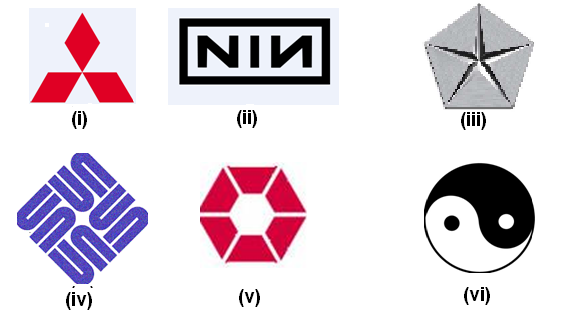
\includegraphics[scale=0.35]{images/logos.png}
\caption{Logos for Exercise~\ref{exercise:symmetries:describesymm}}
\label{logos}
\end{center}
\end{figure}

\section{The dihedral groups}\label{sec:dihedral}

We have investigated the symmetries of equilateral triangle, square, and regular hexagon. But what about other regular polygons: heptagon, octagon, nonagon, decagon, and so on?
\footnote{Recall from geometry that a \emph{regular} polygon has all sides equal and all angles equal}
In this section, we will  take a general look at the symmetries of $n$-sided regular polygons. 

We already know that the symmetries of an n-sided regular polygon will form a group. We define the \term{
nth dihedral group}\index{Group!dihedral} to be the group of 
symmetries of a regular $n$-gon.
\footnote{Just a reminder that ``symmetry'' here means a rigid motion that leaves the $n$-sided polygon invariant.}
  We will denote this group by
$D_n$\label{dihedralgroup}.  

%% Replaced with tikz figure and change to a counterclockwise rotation - TWJ 5/7/2010
\begin{figure}[htb]
\begin{center}
\tikzpreface{permute_motions_ngon}
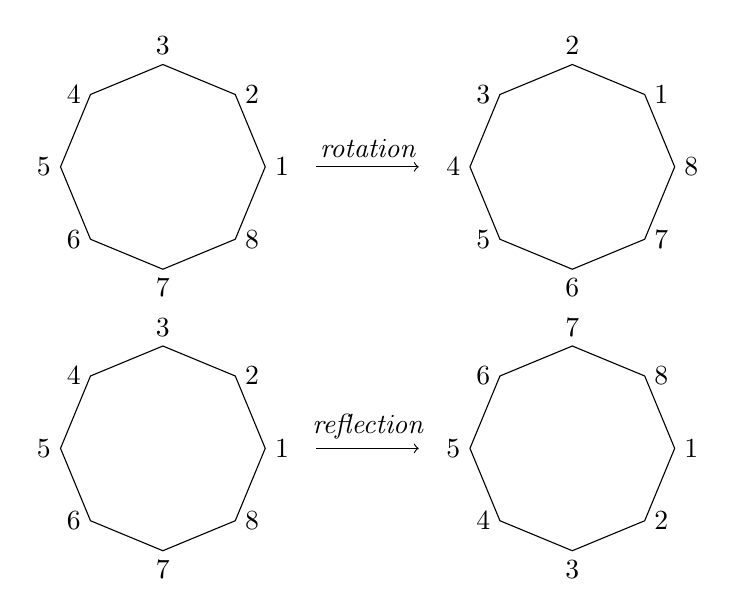
\begin{tikzpicture}[scale=1.3]

\draw (2,0)  +(45:1) node [right] {8} -- +(90:1) node [above] {7} -- +(135:1) node [left] {6} -- +(180:1) node [left] {5} -- +(225:1) node [left] {4} -- +(270:1) node [below] {3} -- +(315:1) node [right] {2} -- +(360:1) node [right] {1} -- cycle;

\draw (-2,0)  +(45:1) node [right] {2} -- +(90:1) node [above] {3} -- +(135:1) node [left] {4} -- +(180:1) node [left] {5} -- +(225:1) node [left] {6} -- +(270:1) node [below] {7} -- +(315:1) node [right] {8} -- +(360:1) node [right] {1} -- cycle;
\draw [->] (-0.5,0) -- (0.5,0);
\node [above] at (0,0) {{\em reflection}};

\draw (2,2.75)  +(45:1) node [right] {1} -- +(90:1) node [above] {2} -- +(135:1) node [left] {3} -- +(180:1) node [left] {4} -- +(225:1) node [left] {5} -- +(270:1) node [below] {6} -- +(315:1) node [right] {7} -- +(360:1) node [right] {8} -- cycle;

\draw (-2,2.75)  +(45:1) node [right] {2} -- +(90:1) node [above] {3} -- +(135:1) node [left] {4} -- +(180:1) node [left] {5} -- +(225:1) node [left] {6} -- +(270:1) node [below] {7} -- +(315:1) node [right] {8} -- +(360:1) node [right] {1} -- cycle;

\draw [->] (-0.5,2.75) -- (0.5,2.75);
\node [above] at (0,2.75) {{\em rotation}};

\end{tikzpicture}
\end{center}
\caption{Rotations and reflections of a regular $n$-gon}
\label{rotations}
\end{figure}


Let us try to count the number of elements of $D_n$ . We can number the vertices of a regular
$n$-gon by $1, 2, \ldots, n$ (Figure~\ref{rotations}).  Any symmetry will move the $n$-gon so that each vertex is replaced by another vertex. Notice that
any vertex can replace the first vertex: so there are exactly $n$ choices to replace the first vertex.
Suppose we
replace  vertex 1 by vertex $k$:  then  vertex 2 must be replaced
either by vertex $k+1$ or by vertex $k-1$, because these are the only vertices next to vertex $k$. So for each of the $n$ choices for replacing vertex 1, there are two choices for replacing vertex 2: which makes $2n$ possible choices altogether. If you think about it, you'll see that once the replacements for vertices 1 and 2 are determined, the entire symmetry is fixed (again, because vertices must remain next to each other).   We summarize our conclusion in
the following proposition.  

 
\begin{prop}{}
The dihedral group, $D_n$, is a group of order $2n$.
\end{prop}
 

Let us try to characterize these $2n$ elements of the dihedral group $D_n$. 
\medskip

First, we know that the elements of the dihedral group includes $n$ rotations:
\[
{\var id}, \frac{360^{\circ} }{n}, 2 \cdot \frac{360^{\circ} }{n},
\ldots, (n-1) \cdot \frac{360^{\circ} }{n}.
\]
We will denote the rotation $360^{\circ} /n$ by $r$. Notice that:
\begin{itemize}
\item
$r \compose r = $ rotation by  $2 \cdot \frac{360^{\circ} }{n}$
\item
$r \compose r \compose r = $ rotation by  $3 \cdot \frac{360^{\circ} }{n}$
\end{itemize}

\noindent
We can generalize this pattern by writing:
\medskip

$r^k = \mbox{ rotation by } k \cdot \frac{360^{\circ} }{n}~~~(k=1,2,3,\ldots),$
\medskip

\noindent
where the notation $r^k$ means that we compose  $r$ with itself $k$ times: $r \compose r \ldots \compose r$.
We can also continue this pattern with $k=0$ and  write:
\medskip

$r^0 = \mbox{ rotation by } 0 \cdot \frac{360^{\circ} }{n} = \var{id}.$
\medskip

We also have
\medskip

$r^n = \mbox{ rotation by } n \cdot \frac{360^{\circ} }{n} = \mbox{ rotation by } 360^{\circ} = {\var id},$
\medskip

\noindent
since rotation by 360 degrees is tantamount to not moving the figure at all.


\begin{exercise}{InverseRot}
\begin{enumerate}[(a)]
\item
Using the above definition of $r^k$, show that $r^k \compose r^m = r^{m+k}$ for any natural numbers $k,m$.
\item
Show that $r^k \compose r^{n-k} = r^{n-k} \compose r^k = {\var id}$
 for $1 < k < n$.  
\item
What does (b) tell us about the inverse of $r^k$?
\end{enumerate}
\end{exercise}

From the above discussion, it should be clear that the $n$ rotations in $D_n$ can be expressed as:
\[{\var id}, r, r^2, \ldots, r^{n-1},\]
where we have included ${\var id}$ since it is ``rotation by 0 degrees'' (as mentioned above, we could also write $\var{id}$ as $r^0$).  This gives us a nice way of characterizing the rotations in $D_n$.  But until now we don't have a nice way of writing the reflections. We'll take care of that now!

We have labeled the vertices of the $n$-gon as $1,2,\ldots,n$. In the following discussion, we will use the letter  $s$ to denote the reflection that leaves the vertex labeled 1  \emph{fixed}, that is, $s(1) = 1$.\footnote{In math books you may also find the termi ``invariant'' instead of ``fixed''.}  Another way of saying the same thing is:  the vertex labeled 1 is ``fixed by'' $s$.

\begin{exercise}{}
\begin{enumerate}[(a)]
\item
Write the reflection $s$  for the pentagon in tableau form.  
\item
How many vertices are fixed by $s$? What are they?
\item
What is $s^2$?  (Recall that $s^2$ means the same as $s \compose s$.)
\end{enumerate}
\end{exercise}

\begin{exercise}{31}
\begin{enumerate}[(a)]
\item
Write the reflection $s$ for the octagon in tableau form. 
\item
How many vertices are fixed by $s$? What are they?
\item
What is $s^2$?
\end{enumerate}
\end{exercise}

By generalizing the arguments used in the preceding exercises, it is possible to prove for any $n$ that:

$$ s^2 = {\var id}.$$

Now we have already shown there are $n$ distinct rotations. Suppose we follow each of these rotations by the reflection $s$: that is, consider the set
\[
S \equiv \{s \compose {\var id}, s \compose r, s \compose r^2,
\ldots, s \compose r^{n-1}\}
\]

It appears that $S$ has $n$ elements: but are these elements distinct? The following exercise provides an answer:

\begin{exercise}{}
Prove the following proposition by filling in the blanks:
\medskip

\noindent \textbf{Proposition.} 
If $0< p,q < n$ and $p \neq q$, then $s \compose r^p$ and $s \compose r^q$ are distinct elements of $D_n$: that is, $s\circ r^p \neq s \compose r^q$.
\medskip

\begin{proof}
\begin{itemize}
\item
 The proof is by contradiction. Given  $0< p,q < n$ and  $p \neq q$, and suppose that $s \compose r^p  \underline{~<1>~} s \compose r^q$
\item
Compose both sides of the equation with $s$, and obtain the equation:  $s \compose (s \compose r^p) =  \underline{~<2>~} $.
\item
By the associative property of composition, this can be rewritten: $(s \compose s) \compose \underline{~<3>~}  =  \underline{~<4>~}$
\item
Since $s \compose s = \underline{~<5>~}$, this can be rewritten: ${\var id} \compose \underline{~<6>~}  =  \underline{~<7>~}$.
\item
Since ${\var id}$ is a group identity, we have: $r^p = \underline{~<8>~}$.
\item
But we have already shown that $r^p$ and $r^q$ are distinct symmetries if $0< p,q < n$ and  $p \neq q$. This is a contradiction.
\item
Therefore we conclude that our supposition was incorrect, and $s \compose r^p  \underline{~<9>~} s \compose r^q$. This completes the proof.
\end{itemize}
\end{proof}
\end{exercise}

\begin{exercise}{33}
Prove the following proposition: 
\medskip

\noindent
\textbf{Proposition}
If $0< q < n$  then $s$ and $s \compose r^q$ are distinct elements of $D_n$: that is, $s \neq s \compose r^q$.
\medskip
\hyperref[sec:symmetries:hints]{(*Hint*)}
\end{exercise}

\begin{exercise}{34}
Fill in the blanks to prove that given any integers $p,q$ with $0< p,q < n$, $s \compose r^p \neq r^q$ :
\begin{itemize}
\item
The proof is by contradiction: so given integers $p,q$ with $0< p,q < n$, we suppose $\underline{~<1>~}$.
\item
By multiplying both sides on the \emph{right} by $r^{n-p}$, we obtain $s \compose r^p \compose \underline{~<2>~} = r^q \compose \underline{~<3>~}$
\item
By associativity, we have $s \compose  \underline{~<4>~} =  \underline{~<5>~}$
\item
Using the fact that \underline{~<6>~} = {\var id}, we obtain $s = \underline{~<7>~}$
\item
The left side of this equation is a reflection, and the right side is a $\underline{~<8>~}$, which is a contradiction.
\item
This contradiction implies that our supposition is incorrect, so  given integers $p,q$ with $0< p,q < n$, we conclude $\underline{~<9>~}$.
\end{itemize}
\end{exercise}

The preceding exercises have shown that the rotations and $\{s, s \compose r, s \compose r^2,
\ldots, s \compose r^{n-1}\}$ are all distinct elements of $D_n$. Since there are $2n$ of these symmetries altogether, and since $D_n$ has  $2n$ elements, we have proved the following:

\begin{prop}{D_elts}
The $2n$ elements of $D_n$ may be listed as: 
\[\{ {\var id}, r, r^2, \ldots, r^{n-1},  s, s \compose r, s\circ r^2, \ldots, s \compose r^{n-1}\},\]
or alternatively  as
\[\{  s^j \compose r^k, ~~(j=0,1;~ k = 0,1,\ldots n-1 \},\]
where we are using the notation:  $s^0 = r^0 = {\var id}$.
\end{prop}

There is actually another way to characterize the elements of $D_n$, as we shall see in the following exercises:

 
\begin{figure}[hbt]
\begin{center}

\tikzpreface{permute_dihedral_four}
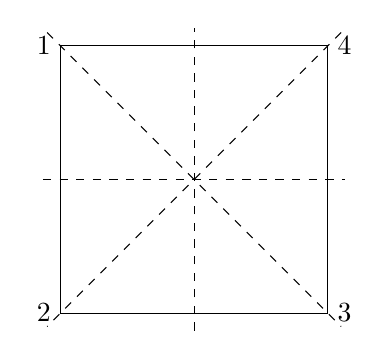
\begin{tikzpicture}[scale=1.2] %% Replaced with tikz figure and change to a counterclockwise rotation - TWJ 5/8/2010

\draw (0,0)  +(45:2) node [right] {4} -- +(135:2) node [left] {1} -- +(225:2) node [left] {2} -- +(315:2) node [right] {3} -- cycle;

\draw[dashed] (0,-1.6) -- (0,1.6);
\draw[dashed] (-1.6,0) -- (1.6,0);
\draw[dashed] (45:2.2) -- (225:2.2);
\draw[dashed] (135:2.2) -- (315:2.2);

\end{tikzpicture}
\end{center}
\caption{Lines of reflection for a square ($D_4)$}
\label{D4}
\end{figure}


\begin{figure}[hbt]  %% Replaced with tikz figure and change to a counterclockwise rotation - TWJ 5/8/2010
\begin{center}
\tikzpreface{permute_reflections_ngon}
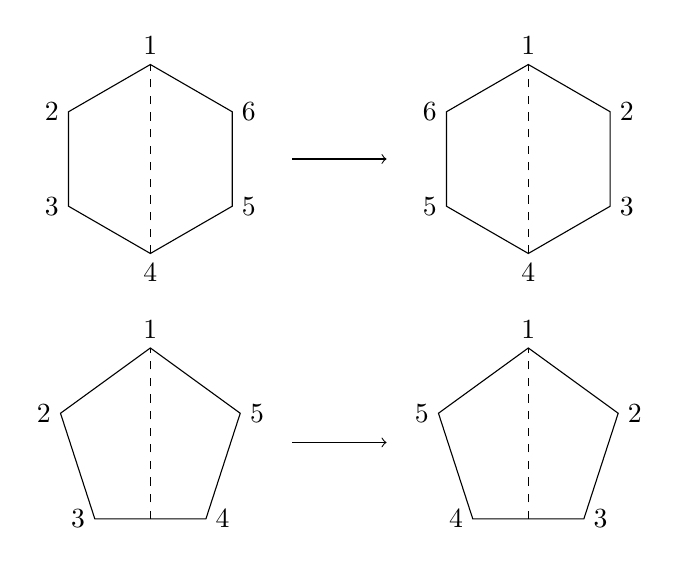
\begin{tikzpicture}[scale=1.2]

\draw (2,0)  +(18:1) node [right] {2} -- +(90:1) node [above] {1} -- +(162:1) node [left] {5} -- +(234:1) node [left] {4} -- +(306:1) node [right] {3} -- cycle;
\draw[dashed] (2,-0.80901) -- (2,1);

\draw (-2,0)  +(18:1) node [right] {5} -- +(90:1) node [above] {1} -- +(162:1) node [left] {2} -- +(234:1) node [left] {3} -- +(306:1) node [right] {4} -- cycle;
\draw[dashed] (-2,-0.80901) -- (-2,1);

\draw [->] (-0.5,0) -- (0.5,0);


\draw (2,3)  +(30:1) node [right] {2} -- +(90:1) node [above] {1} -- +(150:1) node [left] {6} -- +(210:1) node [left] {5} -- +(270:1) node [below] {4}  -- +(330:1) node [right] {3} -- cycle;
\draw[dashed] (2,2) -- (2,4);


\draw (-2,3)  +(30:1) node [right] {6} -- +(90:1) node [above] {1} -- +(150:1) node [left] {2} -- +(210:1) node [left] {3} -- +(270:1) node [below] {4}  -- +(330:1) node [right] {5} -- cycle;
\draw[dashed] (-2,2) -- (-2,4);

\draw [->] (-0.5,3) -- (0.5,3);


\end{tikzpicture}

\end{center}
\caption{Types of  reflections of a regular $n$-gon}
\label{types}
\end{figure}
 


\begin{exercise}{36}
\begin{enumerate}[(a)]
\item
List four reflections of the square in tableau form.
\hyperref[sec:symmetries:hints]{(*Hint*)}
\item
Let $\mu$ be any of the reflections in part (a). What is $\mu \compose \mu$?
\item
How many reflections have no fixed vertices?
\item
How many reflections fix exactly one vertex?
\item
How many reflections fix exactly two vertices?

\end{enumerate}
\end{exercise}


\begin{exercise}{PentagonRefl}
\begin{enumerate}[(a)]
\item
List five reflections of the pentagon in tableau form.
\hyperref[sec:symmetries:hints]{(*Hint*)}
\item
Let $\mu$ be any of the reflections in part (a). What is $\mu \compose \mu$?
\item
How many reflections have no fixed vertices?
\item
How many reflections fix exactly one vertex?
\item
How many reflections fix exactly two vertices?

\end{enumerate}
\end{exercise}

\begin{exercise}{HexagonRefl}
\begin{enumerate}[(a)]
\item
List six reflections of the hexagon in tableau form.
\hyperref[sec:symmetries:hints]{(*Hint*)}
\item
Let $\mu$ be any of the reflections in part (a). What is $\mu \compose \mu$?
\item
How many reflections have no fixed vertices?
\item
How many reflections fix exactly one vertex?
\item
How many reflections fix exactly two vertices?

\end{enumerate}
\end{exercise}

\begin{exercise}{nonagon}
\begin{enumerate}[(a)]
\item 
Complete the second row of the following tableau that represents the reflection of the nonagon that fixes vertex 4:

$$\mu_1 = \begin{pmatrix} 1 & 2 & 3 & 4 & 5 & 6 & 7 & 8 & 9 \\ \_\_ & \_\_ & \_\_ & 4 & \_\_ & \_\_ & \_\_ & \_\_ & \_\_   \end{pmatrix}$$

\item
Complete the second row of the following tableau that represents the reflection of the 10-gon that fixes vertex 4:

$$\mu_2 = \begin{pmatrix} 1 & 2 & 3 & 4 & 5 & 6 & 7 & 8 & 9 & 10  \\ \_\_ & \_\_ & \_\_ & 4 & \_\_ & \_\_ & \_\_ & \_\_ & \_\_ & \_\_   \end{pmatrix}$$


\item 
Complete the second row of the following tableau that represents the reflection of the 10-gon that exchanges vertices 6 and 7:

$$\mu_3 = \begin{pmatrix} 1 & 2 & 3 & 4 & 5 & 6 & 7 & 8 & 9 & 10 \\ \_\_ & \_\_ & \_\_  & \_\_ & \_\_ & 7 & 6 & \_\_ & \_\_ & \_\_  \end{pmatrix}$$

\item
What is $\mu_1 \compose \mu_1$? What is $\mu_2 \compose \mu_2$? What is $\mu_3 \compose \mu_3$?
\end{enumerate}
\end{exercise}

The preceding exercises are generalized to arbitrary $n$ in the following proposition. Although we do not give a complete proof, it is reasonable that we can generalize Exercise~\ref{exercise:symmetries:PentagonRefl} to all \emph{odd} $n$-gons, and we can  generalize Exercise~\ref{exercise:symmetries:HexagonRefl} to all \emph{even} $n$-gons:

\begin{prop}{}
\begin{itemize}
\item
The dihedral group $D_n$ contains $n$ distinct reflections (in addition to $n$ distinct rotations);
\item
For any reflection $\mu \in D_n$, we have $\mu \compose \mu = {\var id}$.
\end{itemize}
\end{prop}

\begin{exercise}{41}
\begin{enumerate}[(a)]
\item
Based on results we've shown, prove that $s \compose r^p$ must be a reflection, for $0 < p < n$.
\item
Using part (a) and other results we've shown, show that $(s \compose r^p) \compose (s \compose r^p) = {\var id}$.
\hyperref[sec:symmetries:hints]{(*Hint*)}
\item
Using part (b) and composing on the left by $r^{n-p} \compose s$, show that $  r^{n-p} \compose s = s \compose r^p$  for $0< p < n$.
\end{enumerate}
\end{exercise}

All of our results on dihedral groups can now be summarized in the following proposition:

\begin{prop}{Dn_generator_theorem}
Every element of the group $D_n$, $n \geq 3$, consists of all compositions of the two 
elements $r$ and $s$, satisfying the relations:
\begin{enumerate}[(a)]
\item
$r^n  = {\var id}$
\item
$s^2  = {\var id} $
\item
$ r^p \compose s  = s \compose  r^{n-p} \mbox{ for } 0<p<n$.
\end{enumerate}
\end{prop}
 
Proposition~\ref{proposition:symmetries:Dn_generator_theorem} enables us to compute any composition of elements of $D_n$ directly, without 
the need of tableau form:

\begin{example}{compref}
In $D_5$, to compute $(s \compose r^3) \compose (s \compose r^4)$ we have (using Proposition~\ref{proposition:symmetries:Dn_generator_theorem} and associativity):  

\begin{align*}
(s \compose r^3) \compose (s \compose r^4) &= s \compose (r^3 \compose s) \compose r^4 \mbox{     by associativity}\\
&= s \compose (s \compose r^2) \compose r^4 \mbox{      by Prop.~\ref{proposition:symmetries:Dn_generator_theorem}(c)}\\
&= (s \compose s) \compose r \compose r^5 \mbox{      by  associativity}\\
&= {\var id} \compose r \compose {\var id} \mbox{      by Prop.~\ref{proposition:symmetries:Dn_generator_theorem}(a) and (b)}\\
&= r
\end{align*}
\end{example}
In fact, following the method of Example\ref{example:symmetries:compref} it is possible to derive a general formula for the composition of two reflections. Such a formula may be very useful in certain situations: for instance, in the following exercises.

 \begin{exercise}{44}
Using only associativity and Proposition~\ref{proposition:symmetries:Dn_generator_theorem}, complete the entire Cayley table for $D_4$.  Remember, there is a row and a column for each element of $D_4$. List the elements as indicated in Proposition~\ref{proposition:symmetries:D_elts}. You don't need to show all your computations. \emph{(But don't use tableau form--no cheating!)} 
\end{exercise}

 \begin{exercise}{}
Using only associativity and Proposition~\ref{proposition:symmetries:Dn_generator_theorem}, complete the entire Cayley table for $D_5$.  You don't need to show all your computations. \emph{(But don't use tableau form -- no cheating!)} 
\end{exercise}

\section{For further investigation}
In this chapter, we have looked at the groups involved with symmetries of plane figures. But really, there is no need to restrict ourselves to two dimensions. Three-dimensional regular figures (such as the tetrahedron, cube, icosahedron, and dodecahedron) also have symmetry groups associated with them. These symmetry groups also make for fascinating study.

Neither do we need to restrict ourselves to symmetries of objects. The symmetries of \emph{patterns} also play an important role in art and architecture.  For instance, every possible regular repeating pattern that can be put on wallpaper (or used as floor tiling) is associated with a symmetry group. It turns out that there are exactly 17 of these symmetry groups: they are called the \emph{wallpaper groups}.\index{Wallpaper groups}\index{Group!wallpaper} For an excellent elementary reference on this subject, I highly recommend ``17 Plane Symmetry Groups" by Anna Nelson, Holli Newman, and Molly Shipley, available on the web (as of January 2014) at \url{http://caicedoteaching.files.wordpress.com/2012/05/nelson-newman-shipley.pdf}. 

In physics, symmetry groups are used to describe the regular three-dimensional patterns associated with crystals. Many references for the crystallographic groups can also be found on the web: one I recommend is "Crystallographic Point Groups (short review)" by Mois I. Aroyo, available on the web at: \url{http://www.crystallography.fr/mathcryst/pdf/uberlandia/Aroyo_Point.pdf}.


\section{An unexplained miracle} \label{sec:miracle}

It's good for us to step back for a moment and take stock of what we've accomplished so far. We'll begin with some exercises.

\begin{exercise}{46}
\begin{enumerate}[(a)]
\item
Give the Cayley table for the integers mod 4 under addition.
\item 
Give the Cayley table for the four rotations of the square (4-sided polygon).  You may use $r$ to denote rotation by $90$ degrees, so that the rotations will be $\{ {\var id}, r, r^2, r^3  \}$.
\item 
Give the Cayley table for the four complex $4'{th}$ roots of unity. You may use $z$ to denote cis($\pi / 2$) so that the roots will be $\{ 1, z, z^2, z^3 \}$.
\item
Do you see any connection between your answers to (a), (b), and (c) above?
\end{enumerate}
\end{exercise}
%
%\begin{exercise}{eqmod5}
%\begin{enumerate}[(a)]
%\item
%Consider equivalence mod 5 as an equivalence relation on the natural numbers. Write down the 5 equivalence classes for this equivalence relation.
%\hyperref[sec:symmetries:hints]{(*Hint*)}
%\item
%Consider the group $D_5$, and let $r \in D_5$ be rotation by 72 degrees. Define an equivalence relation $\sim$ on the natural numbers as follows: we say $n\sim m$ if $r^n = r^m$. (For instance, $3 \sim 8$ since rotation by $3 \cdot 72 = 216$ degrees is the same as rotation by $8 \cdot 72 = 576 = 216 + 360$ degrees). Write down the 5 equivalence classes for the equivalence relation $~$.
%\end{enumerate}
%\end{exercise}
%\medskip

Exercise~\ref{exercise:symmetries:46} show a deep connection between three extremely diverse concepts that arose from three totally different fields of study:
\begin{itemize}
\item
Arithmetic mod $n$, which first arose from the study of the natural numbers and their divisibility properties;
\item
The $n$’th complex roots of unity, a concept that arose from the study of roots of polynomials.
\item
The rotations of a regular $n$-gon, which is a purely geometrical phenomenon.
\end{itemize}

We express the amazing similarity between these three diverse concepts by saying that they are all described by the ``same'' group. (The technical term for this is ``isomorphism'': we will study this concept in detail in Chapter~\ref{isomorph}.)

Take a moment to appreciate how incredible this is. How is it that three concepts with totally different backgrounds and completely different applications end up being described in exactly the same way?

But the wonders do not stop there. It turns out that an infinite version of this same group is an important part of the so-called Standard Model of quantum physics, that is used to explain the existence of particles such as electrons, protons, and neutrons. How is it that a mathematical structure introduced by an $18^{th}$ century mathematician
\footnote{This mathematician was Leonhard Euler (1707-1783). The integers mod $n$ were further developed by Carl Friedrich Gauss (1777-1855).}
 to study integer division could end up influencing the theory of elementary particles that were not even dreamed of in the $18^{th}$ century?

This mystical unity of description across widely different phenomena says something very profound about the universe. Galileo
\footnote{Galileo Galilei, Italian physicist (1564-1642), whose work on the motion of objects was foundational to the later work of Isaac Newton.}
 expressed it this way: "Mathematics is the language with which God has written the universe." When Galileo said this, his mathematics consisted of little more than what today we would call ``high school algebra'' -- he had not an inkling of abstract algebra. But what Galileo expressed based on his limited mathematics has turned been fulfilled with a vengeance by abstract algebra.
 
Physicist Eugene Paul Wigner\footnote{1902-1995} won the 1963 Nobel Prize in Physics, in part because of his application of the theory of groups to quantum physics. In 1960 Wigner wrote a famous paper called "the Unreasonable Effectiveness of Mathematics in the Natural Sciences,"
\footnote{The paper can be found at:  http://www.dartmouth.edu/$\sim$matc/MathDrama/reading/Wigner.html}
 in which he states: "The miracle of the appropriateness of the language of mathematics for the formulation of the laws of physics is a wonderful gift which we neither understand nor deserve." To this day, apparently no physicist or mathematician has yet offered a satisfactory explanation for Wigner's ``miracle''.

